\documentclass[14pt,a4paper]{article}
\usepackage[utf8]{inputenc}
\usepackage[russianb]{babel}
\usepackage[left=1.5cm,right=1.5cm,top=2cm,bottom=2.5cm]{geometry}
\usepackage{setspace}
\usepackage{indentfirst}
\usepackage{amssymb}
\usepackage{amsmath}
\usepackage{bm}

\usepackage{array}
\usepackage[pdftex]{graphicx}
\usepackage{comment}
\usepackage[table,xcdraw]{xcolor}


\usepackage{verbatim}


\graphicspath{{images/}}
\renewcommand{\baselinestretch}{1.3}

\begin{document}

Квадрат разлинован на $N \times N$ клеток $(1 < N < 30)$. Исполнитель
Робот может перемещаться по клеткам, выполняя за одно перемещение
одну из двух команд: \textbf{вправо} или \textbf{вниз}. По команде
\textbf{вправо} Робот перемещается в соседнюю правую клетку, по
команде \textbf{вниз} -- в соседнюю нижнюю. Квадрат ограничен
внешними стенами. Между соседними клетками квадрата также могут быть
внутренние стены. Сквозь стену Робот пройти не может. Перед каждым
запуском Робота в каждой клетке квадрата лежит монета достоинством от
1 до 100. Посетив клетку, Робот забирает монету с собой; это также
относится к начальной и конечной клеткам маршрута Робота. В
<<угловых>> клетках поля -- тех, которые справа и снизу ограничены
стенами, Робот не может продолжать движение, поэтому накопленная
сумма считается итоговой. Таких конечных клеток на поле может быть
несколько, включая правую нижнюю клетку поля. При разных запусках
итоговые накопленные суммы могут различаться. Определите максимальную
и минимальную денежные суммы, среди всех возможных итоговых сумм,
которые может собрать Робот, пройдя из левой верхней клетки в
конечную клетку маршрута. В ответе укажите два числа – сначала
максимальную сумму, затем минимальную.

Исходные данные представляют собой электронную таблицу размером $N
\times N$, каждая ячейка которой соответствует клетке квадрата.
Внутренние и внешние стены обозначены утолщёнными линиями.

\textit{Пример входных данных}

\begin{center}
    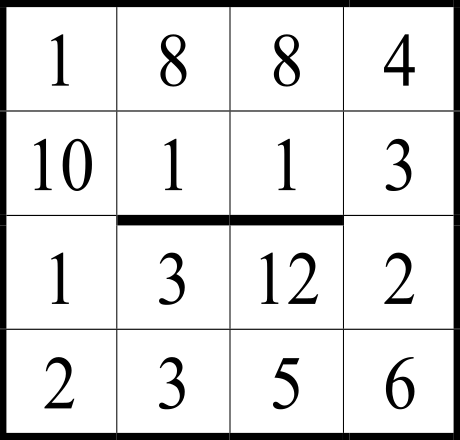
\includegraphics[width=0.2\textwidth]{example.png}
\end{center}

\end{document}
